% Source: graduate-coursework/Sp26/CSCE775/course_notes/quiz_2_cheatsheet.tex

\documentclass[border=4pt]{standalone}
\usepackage{amsmath, amssymb}
\usepackage{tikz}
\usepackage{xcolor}
\usetikzlibrary{arrows.meta, positioning, calc}

\definecolor{garnet}{HTML}{73000A}
\definecolor{black90}{HTML}{363636}
\definecolor{black70}{HTML}{5C5C5C}
\definecolor{atlantic}{HTML}{466A9F}
\definecolor{congaree}{HTML}{1F414D}
\definecolor{horseshoe}{HTML}{65780B}
\definecolor{rose}{HTML}{CC2E40}
\definecolor{honeycomb}{HTML}{A49137}
\definecolor{grass}{HTML}{CED318}
\definecolor{sandstorm}{HTML}{FFF2E3}
\definecolor{black10}{HTML}{ECECEC}

\newcommand{\mathbox}[2]{%
\begin{tcolorbox}[colback=sandstorm, colframe=garnet, title={\scriptsize\bfseries\color{white}#1}, coltitle=white, colbacktitle=garnet, toptitle=1pt, bottomtitle=1pt]
#2
\end{tcolorbox}
}
\newcommand{\conceptbox}[2]{%
\begin{tcolorbox}[colback=atlantic!5, colframe=atlantic, title={\scriptsize\bfseries\color{white}#1}, coltitle=white, colbacktitle=atlantic, toptitle=1pt, bottomtitle=1pt]
#2
\end{tcolorbox}
}
\newcommand{\warnbox}[1]{%
\begin{tcolorbox}[colback=rose!8, colframe=rose, boxrule=0.8pt]
\textcolor{rose}{\textbf{!}} #1
\end{tcolorbox}
}

\def\columnseprulecolor{\color{black!20}}

\begin{document}
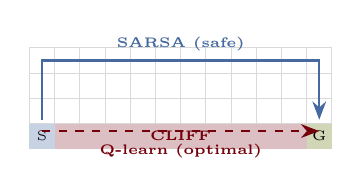
\begin{tikzpicture}[scale=0.32, every node/.style={font=\tiny}]
    \foreach \x in {0,...,11} \foreach \y in {0,...,3}
        \draw[black!15] (\x,\y) rectangle (\x+1,\y+1);
    \foreach \x in {1,...,10}
        \fill[garnet!25] (\x,0) rectangle (\x+1,1);
    \node[garnet, font=\tiny\bfseries] at (6, 0.5) {CLIFF};
    \fill[atlantic!30] (0,0) rectangle (1,1);
    \node at (0.5,0.5) {S};
    \fill[horseshoe!30] (11,0) rectangle (12,1);
    \node at (11.5,0.5) {G};
    \draw[-{Stealth}, atlantic, thick] (0.5,1.15) -- (0.5,3.5) -- (11.5,3.5) -- (11.5,1.15);
    \node[atlantic, above, font=\tiny\bfseries] at (6,3.5) {SARSA (safe)};
    \draw[-{Stealth}, garnet, thick, dashed] (0.5,0.7) -- (11.5,0.7);
    \node[garnet, below, font=\tiny\bfseries] at (6,0.55) {Q-learn (optimal)};
\end{tikzpicture}
\end{document}
